\documentclass[12pt]{article}
\usepackage[utf8]{inputenc}
\usepackage{hyperref}
\usepackage{tikz}
\usepackage{graphicx}
\usetikzlibrary{decorations.pathreplacing}
\usetikzlibrary{patterns, positioning, arrows.meta}

\title{On Memory Architecture}
\author{Shaan Fulton}
\date{\today}

\begin{document}

\maketitle

We know how to represent information as bits. We also know that we can represent both data and instructions as bits (this is von Neumann architecture, see \texttt{the-stored-program}).

But how does this actually work in practice? Do we just have a massive list of one's and zero's to represent our instructions and variables? Yes, we do. Memory (and storage, for that matter) looks like this:

\begin{center}
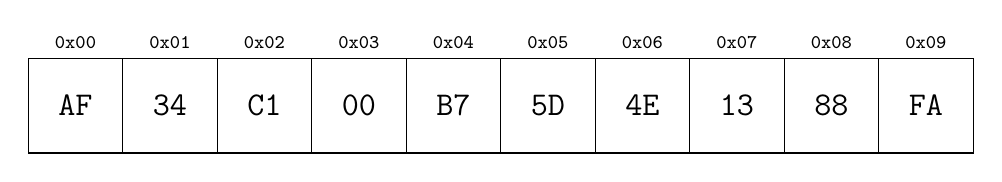
\begin{tikzpicture}
  \def\cellsize{1.2cm}
  \foreach \i/\addr/\data in {
    0/0x00/AF,
    1/0x01/34,
    2/0x02/C1,
    3/0x03/00,
    4/0x04/B7,
    5/0x05/5D,
    6/0x06/4E,
    7/0x07/13,
    8/0x08/88,
    9/0x09/FA
  }{
    % Draw cell
    \draw (\i*\cellsize,0) rectangle ++(\cellsize,\cellsize);
    % Byte data inside
    \node at (\i*\cellsize+0.5*\cellsize,0.5*\cellsize) {\large\texttt{\data}};
    % Address above
    \node[anchor=south] at (\i*\cellsize+0.5*\cellsize,\cellsize) {\scriptsize\texttt{\addr}};
  }
\end{tikzpicture}
\end{center}

Memory is byte addressable. That means every byte (256 combinations, 8 bits, 2 hexadecimal digits) has an address.

\begin{quote}
``Why not make things bit addressable instead?''
\end{quote}

We could. But memory addresses can only be so long. Our CPU gets data through a memory bus (more in this below). These memory buses are only so long. For example, if we have a 128-bit memory address but our CPU memory bus is only 8-bits, it will take 16 operations just to get our address processed by the CPU so that we might be able to visit it. This is terribly inefficient.

If we made things bit addressable, a reasonable 32-bit memory address would allow for $4,294,967,296$ combinations. This means we would be able to address $4,294,967,296$ bits, or $536,870,912$ bytes, which is about 500 MB.

That sucks. That means the maximum RAM we can have in our system is 500 MB. Conversely, if we make our system byte addressable, we up that to 4 GB. Much better.

\section*{The Memory Bus}

So we have this massive array of cells, each containing one byte, with a little address fixed to it. We'll assume we're working on a 32-bit address bus (32-bit addresses, a 32-bit system, etc.). But how do we actually use this array?

Our CPU has to perform its minimal operation set so that we can compose and execute all sorts of programs. But it needs to get its instructions and data from memory somehow. The CPU uses a CPU bus to accomplish this.

Think of the CPU bus like a fixed width vacuum. In our system, it can suck up 32 bits of memory at a time.

\begin{center}
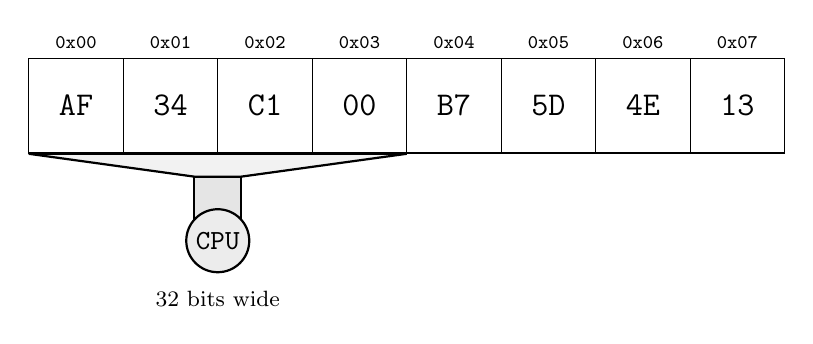
\begin{tikzpicture}
  \def\cellsize{1.2cm}
  \def\ncells{8}
  \def\buswidth{4} % number of bytes for 32 bits
  \def\tubewidth{0.6cm}
  \def\tubeheight{0.8cm}
  \def\trapezheight{0.3cm}

  % Draw memory cells
  \foreach \i/\addr/\data in {
    0/0x00/AF,
    1/0x01/34,
    2/0x02/C1,
    3/0x03/00,
    4/0x04/B7,
    5/0x05/5D,
    6/0x06/4E,
    7/0x07/13
  }{
    \draw (\i*\cellsize,0) rectangle ++(\cellsize,\cellsize);
    \node at (\i*\cellsize+0.5*\cellsize,0.5*\cellsize) {\large\texttt{\data}};
    \node[anchor=south] at (\i*\cellsize+0.5*\cellsize,\cellsize) {\scriptsize\texttt{\addr}};
  }

  % Draw trapezoid for the bus under the first 4 cells
  \draw[thick, fill=gray!10]
    (0, -0.01) -- % left top
    (\buswidth*\cellsize, -0.01) -- % right top
    (\buswidth*\cellsize/2 + \tubewidth/2, -\trapezheight) -- % right bottom
    (\buswidth*\cellsize/2 - \tubewidth/2, -\trapezheight) -- % left bottom
    cycle;

  % Label "32 bits wide" under the trapezoid
  \node at (\buswidth*\cellsize/2, -1.85) {\footnotesize 32 bits wide};

  % Draw rectangle (tube) leading down from the trapezoid
  \draw[thick, fill=gray!20]
    (\buswidth*\cellsize/2 - \tubewidth/2, -\trapezheight) rectangle ++(\tubewidth, -\tubeheight);

  % Draw CPU circle below tube
  \draw[thick, fill=gray!15]
    (\buswidth*\cellsize/2, -\trapezheight - \tubeheight - 0.4) circle [radius=0.4];
  \node at (\buswidth*\cellsize/2, -\trapezheight - \tubeheight - 0.4) {\texttt{CPU}};

\end{tikzpicture}
\end{center}

\subsection*{Memory Alignment}

Because the CPU is sucking up 32 bits at a time, or 4 bytes, that means it can read a whole integer at once (most integers are represented with 32 bits)! That's very convenient. We can easily pull in an integer to do operations on it and then spit it back out all in single swoops. It can also read 4 characters at once (ASCII characters are just 8 bits or 1 byte)!

But there's a little caveat to all this. The CPU memory bus isn't really like a free-floating vacuum that can align itself to any address. The actual hardware more closely resembles a set of drawers where each drawer contains 4 bytes (imagine four folders, or dividers). And so in reality, the CPU memory bus can't read addresses 2 to 5 or 3 to 6 in one go, because these would be folders between two seperate drawers (drawers containing 0 to 3 and 4 to 7 respectively).

\begin{center}
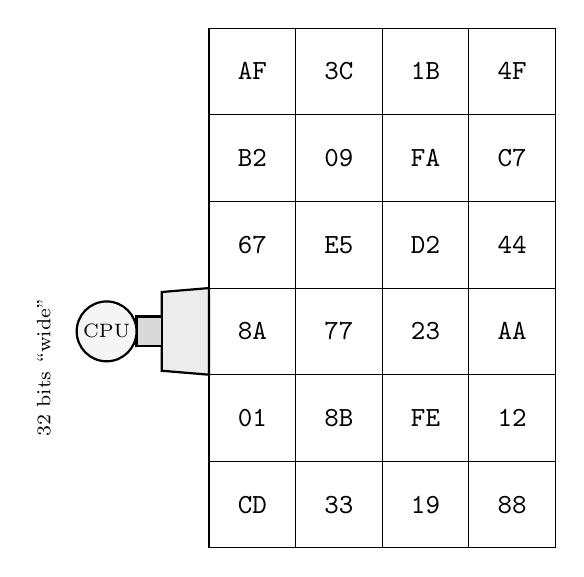
\begin{tikzpicture}
  % Size settings
  \def\cellsize{1.1}
  \def\nrows{6}
  \def\ncols{4}
  \def\busrow{3} % which row is read by the bus (0=top)

  % Hard-coded hex data for each row (must match nrows x ncols)
  \def\memA{{"AF","3C","1B","4F"}}
  \def\memB{{"B2","09","FA","C7"}}
  \def\memC{{"67","E5","D2","44"}}
  \def\memD{{"8A","77","23","AA"}}
  \def\memE{{"01","8B","FE","12"}}
  \def\memF{{"CD","33","19","88"}}
  \def\alldata{{\memA,\memB,\memC,\memD,\memE,\memF}}

  % Draw memory cells with hex contents
  \foreach \row in {0,...,5} {
    \foreach \col in {0,...,3} {
      \draw (\col*\cellsize, -\row*\cellsize) rectangle ++(\cellsize, -\cellsize);
      \pgfmathsetmacro\cellcontent{\alldata[\row][\col]}
      \node at (\col*\cellsize+0.5*\cellsize, -\row*\cellsize-0.5*\cellsize) {\texttt{\cellcontent}};
    }
  }

  % Trapezoid for bus, on the left of the selected row
  \def\trapin{0.6} % how much the left side juts out
  \coordinate (T1) at (-\trapin, -\busrow*\cellsize-0.05);
  \coordinate (T2) at (0, -\busrow*\cellsize);
  \coordinate (T3) at (0, -\busrow*\cellsize-\cellsize);
  \coordinate (T4) at (-\trapin, -\busrow*\cellsize-\cellsize+0.05);
  \draw[thick, fill=gray!15] (T1)--(T2)--(T3)--(T4)--cycle;

  % Rectangle "tube" (small, centered on trapezoid)
  \def\tubew{0.32}
  \def\tubeh{0.38}
  \coordinate (TubeTL) at (-\trapin-\tubew, -\busrow*\cellsize-0.5*\cellsize+\tubeh/2);
  \draw[thick, fill=gray!30]
    (TubeTL) rectangle ++(\tubew, -\tubeh);

  % Large CPU circle at end of tube
  \def\cpurad{0.38}
  \coordinate (CPUcenter) at (-\trapin-\tubew-\cpurad, -\busrow*\cellsize-0.5*\cellsize);
  \draw[thick, fill=gray!08] (CPUcenter) circle (\cpurad);
  \node at (CPUcenter) {\scriptsize CPU};

  % Vertical label for the bus width
  \node[anchor=east, font=\scriptsize, rotate=90]
    at (-\trapin-1.5, -\busrow*\cellsize-0.0*\cellsize) {32 bits ``wide''};

\end{tikzpicture}
\end{center}

To accomodate this architecture, we actually make sure that our data is stored in ``alignment'' with these drawers.

We could totally ignore this and have an integer, for example, stretching between two drawers. But then we would need to make two attempts at getting that integer out of memory. Too slow! And so our memory ends up looking a little like this, with padding wherever we do not fill up an entire 4 byte drawer (yes, it ends up wasting space, but it is faster):

\begin{center}
\vspace{1em}
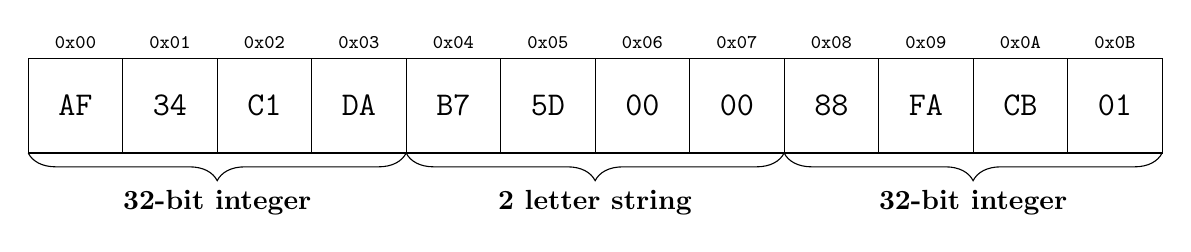
\begin{tikzpicture}
  \def\cellsize{1.2cm}
  \foreach \i/\addr/\data in {
    0/0x00/AF,
    1/0x01/34,
    2/0x02/C1,
    3/0x03/DA,
    4/0x04/B7,
    5/0x05/5D,
    6/0x06/00,
    7/0x07/00,
    8/0x08/88,
    9/0x09/FA,
    10/0x0A/CB,
    11/0x0B/01
  }{
    \draw (\i*\cellsize,0) rectangle ++(\cellsize,\cellsize);
    \node at (\i*\cellsize+0.5*\cellsize,0.5*\cellsize) {\large\texttt{\data}};
    \node[anchor=south] at (\i*\cellsize+0.5*\cellsize,\cellsize) {\scriptsize\texttt{\addr}};
  }
  % Bracket for the first integer (0-3)
  \draw[decorate,decoration={brace,amplitude=10pt,mirror}]
    (0*\cellsize,0) -- (4*\cellsize,0)
    node[midway,below=10pt] {\textbf{32-bit integer}};
  % Bracket for the 2-character string + 2 bytes padding (4-7)
  \draw[decorate,decoration={brace,amplitude=10pt,mirror}]
    (4*\cellsize,0) -- (8*\cellsize,0)
    node[midway,below=10pt] {\textbf{2 letter string}};
  % Bracket for the second integer (8-11)
  \draw[decorate,decoration={brace,amplitude=10pt,mirror}]
    (8*\cellsize,0) -- (12*\cellsize,0)
    node[midway,below=10pt] {\textbf{32-bit integer}};
\end{tikzpicture}
\vspace{1em}
\end{center}

\section*{Memory Locations}

We are very close to understanding how memory works on a computer. But there are some additional details. For instance: do we really just store \textbf{everything} in one massive line, sort of just stacking as we go?

We could. Say we start up a program and grant it a section of memory. Maybe we'll dump all the instructions into memory first, then we'll dump global variables that won't need more space as our application progresses, and lastly we'll dump everything else that comes up as we go through the program (so think local variables and arrays that grow and shrink).

Our memory might look something like this:

\begin{center}
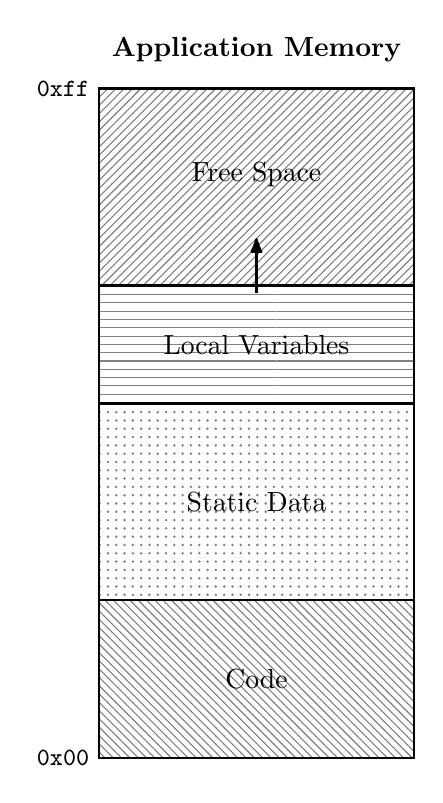
\begin{tikzpicture}[
    section/.style={draw, thick, minimum width=4cm, anchor=north west},
    addr/.style={font=\ttfamily\small},
    arrow/.style={thick, -{Latex[round]}}
]

% Section boundaries -- make Free Space larger
\def\topY{0}
\def\freeY{-2.5}     % Enlarged Free Space section
\def\localY{-4.0}
\def\staticY{-6.5}
\def\codeY{-8.5}

% Main rectangle (memory) exactly to the end of "Code"
\draw[thick] (0,\topY) rectangle (4,\codeY);

% Sections with patterns (classic TikZ patterns)
\draw[section, pattern=north east lines, pattern color=gray] (0,\topY) rectangle (4,\freeY);
\node at (2,{\topY-1.1}) {Free Space};

\draw[section, pattern=horizontal lines, pattern color=gray] (0,\freeY) rectangle (4,\localY);
\node at (2,{\freeY-0.75}) {Local Variables};

\draw[section, pattern=dots, pattern color=gray] (0,\localY) rectangle (4,\staticY);
\node at (2,{\localY-1.25}) {Static Data};

\draw[section, pattern=north west lines, pattern color=gray] (0,\staticY) rectangle (4,\codeY);
\node at (2,{\staticY-1}) {Code};

% Arrow from Local Variables upwards into Free Space
\draw[arrow] (2,\freeY-0.1) -- (2,{\freeY+0.6});

% Title
\node[font=\bfseries] at (2,0.5) {Application Memory};

% Memory addresses outside on the left (top and bottom of box)
\node[addr, anchor=east] at (0,\topY) {0xff};
\node[addr, anchor=east] at (0,\codeY) {0x00};

\end{tikzpicture}
\end{center}

So our little application is running! We pile on the local variables from a function that works on a massive string. And then some more from an advanced physics simulation function. And then more from another massive string manipulator. The ones from this massive string manipulator we want to hold on to, we'll need it later. But as we return to our physics simulation, and return its data, we determine we don't need that space anymore. So we could just store the fact that there's free space in that area now.

But wait. Now we have to keep track of all these little gaps in our data where there's free space. And then whenever we add more things to memory we have to literally iterate over all those gaps to find a spot that works for our piece of data. And my goodness, imagine if we find a spot for a local frame in between other memory areas, and then need to extend that local frame! Now we have to move all that local frame's data to the top of our stack so it can extend freely! This is extremely innefficient, and seeing why is critical to understanding why we store memory the way we actually do.

The key idea here is this: 

\begin{quote}
\textbf{``Local function frame memory is different from long term allocated memory.''}
\end{quote}
The former is quite easy to deal with. We can stack as we get more data, and then simply wipe the stack and move ourselves back down to the last frame and continue stacking from there. That's because once we're done with a local frame we really don't need that data anymore, and we also only go to one local frame at a time, so we just move our little pointer around up and down as we add and remove local frames.

\begin{center}
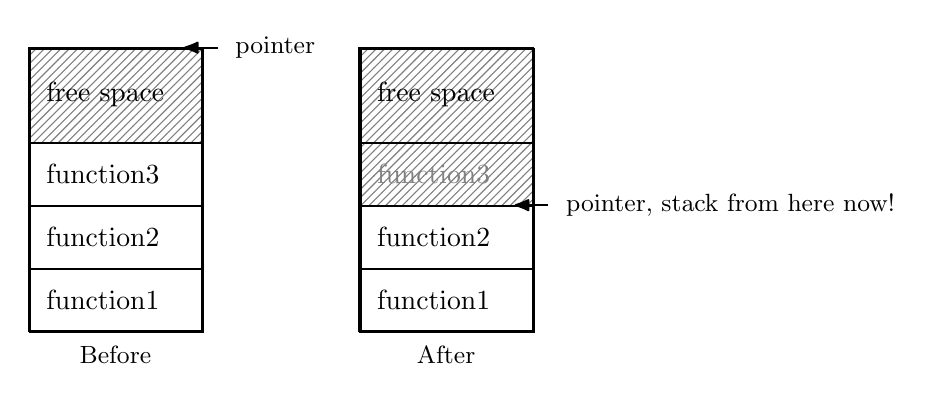
\begin{tikzpicture}[
    section/.style={draw, thick, minimum width=2.2cm, anchor=north west},
    wiped/.style={pattern=north east lines, pattern color=gray},
    framefont/.style={font=\normalsize},
    pointer/.style={thick, -{Latex[round]}, shorten >=2pt},
    labelfont/.style={font=\small}
]

% Frame heights
\def\freeheight{1.2}
\def\frameheight{0.8}
\def\nframes{3}
\def\stackA{0}
\def\stackB{4.2}
\def\stackwidth{2.2}
\pgfmathsetmacro{\stackheight}{\freeheight+\nframes*\frameheight}

% Draw Stack A (Before)
\node[section, wiped, minimum height=\freeheight cm] (Afree) at (\stackA,0) {};
\node[framefont, anchor=west] at (\stackA+0.1,0-0.5*\freeheight) {free space};
\foreach \i/\fname in {0/function3, 1/function2, 2/function1} {
    \pgfmathsetmacro{\y}{-\freeheight-\i*\frameheight}
    \node[section, minimum height=\frameheight cm] (A\i) at (\stackA,\y) {};
    \node[framefont, anchor=west] at (\stackA+0.1,\y-0.5*\frameheight) {\fname};
}
\draw[thick] (\stackA,0) rectangle ++(\stackwidth,-\stackheight);

% Draw Stack B (After)
\node[section, wiped, minimum height=\freeheight cm] (Bfree) at (\stackB,0) {};
\node[framefont, anchor=west] at (\stackB+0.1,0-0.5*\freeheight) {free space};
\foreach \i/\fname in {0/function3, 1/function2, 2/function1} {
    \pgfmathsetmacro{\y}{-\freeheight-\i*\frameheight}
    \ifnum\i=0
        \node[section, wiped, minimum height=\frameheight cm] (B\i) at (\stackB,\y) {};
        \node[framefont, gray, anchor=west] at (\stackB+0.1,\y-0.5*\frameheight) {\fname};
    \else
        \node[section, minimum height=\frameheight cm] (B\i) at (\stackB,\y) {};
        \node[framefont, anchor=west] at (\stackB+0.1,\y-0.5*\frameheight) {\fname};
    \fi
}
\draw[thick] (\stackB,0) rectangle ++(\stackwidth,-\stackheight);

% Pointer for Stack A (top of free space, so at y=0)
\draw[pointer] (\stackA+\stackwidth+0.2,0) -- ++(-0.5,0);
\node[labelfont, anchor=west] at (\stackA+\stackwidth+0.3,0) {pointer};

% Pointer for Stack B (top of function2, which is just below function3, so y=-\freeheight-\frameheight)
\draw[pointer] (\stackB+\stackwidth+0.2, {-\freeheight-\frameheight}) -- ++(-0.5,0);
\node[labelfont, anchor=west] at (\stackB+\stackwidth+0.3, {-\freeheight-\frameheight}) {pointer, stack from here now!};

% Labels below
\node[labelfont] at (\stackA+0.5*\stackwidth,-\stackheight-0.3) {Before};
\node[labelfont] at (\stackB+0.5*\stackwidth,-\stackheight-0.3) {After};

\end{tikzpicture}
\end{center}

The latter is a bit more involved. We need to store a list of where all the free spaces are as we free up data, and shift things around as we extend them. For instance, if we create an array of 20 integers, and later one want to store another 10 integers on the end of that, it would require us to do a bunch of shifting if there's no space on either side. We would have to copy all 20 integers and move them to a larger spot... which means searching through our free list for that larger spot... it's quite involved.

We need this sort of storage. But it's clearly something we'll handle differently from how we handle local function frame storage.

And so: because this long term allocated and reallocated data is more complex to store than short term one time function frame data, we actually create two expanding memory locations...

\subsection*{The Heap and The Stack}

The first of these is the stack. The stack is for our local function frames. The second is the heap. The heap is for this longer term allocated and re-allocated memory. It's data that has to exist between function frames, but is still constantly growing and shifting, unlike static data.

\begin{quote}
{\scriptsize
\textbf{Brief tangent in pedagogy}: Most courses teach the heap and stack by simply explaining what they are and what data they store. This is brute force memorization. The insight of the approach we've taken here is that we're arriving upon it as if inventing it, thus we understand precisely the reason for and beauty of its existence.
}
\end{quote}

And so here it is. Modern memory location architecture:

\begin{figure}[htbp]
    \centering
    \includegraphics[width=0.5\textwidth]{memory-locations.jpg}
    \caption{The Memory Locations}
    \label{fig:memory-locations}
\end{figure}

\begin{table}[h!]
\centering
\begin{tabular}{|l|l|}
\hline
\textbf{Location} & \textbf{What is stored} \\
\hline
Stack & Local variables, function calls \\
Heap & Dynamically allocated memory \\
Data Segment & Global/static variables \\
Code Segment & Program instructions \\
\hline
\end{tabular}
\end{table}

\end{document}

